\section{Inference Rules}
\label{sec:appendix:inference-rules}
In Figure~\ref{fig:inference}, we provide a set of rules that can be used to determining the constraints and guarantees associated with a specification.
We represent
\[ 
X \odot Y : (E, \epsilon, \delta) \equiv \Pr\left(| \E[X] \odot \E[Y] - E | \geq \epsilon \right) \leq \delta
\]
where $\odot$ represents a binary operator.
Constraints are represented in curly brackets $\{ \}$.
%\pmcomment{Need to explain that constraints carry over in missing cases in Figure!\ref{fig:inference}}

%\pmcomment{Add proofs here for inference rules.}
The proof of correctness for each inference rule starts from the assumptions above the horizontal line and derives the assertions below. 
These proofs ise ideas similar to those in \cite{bastani2019probabilistic}.
We reproduce the proofs in Appendix~\ref{sec:appendix:constraint:proofs} here for completeness.
%We provide them here for completeness.
Note that the assertions in the base case (elementary subexpressions) can be arrived at by applying the Adaptive Hoeffding INequality, ($\rm{AIN}$). 

\begin{figure}[!htbp]
%\begin{minipage}{\textwidth}
\centering
\[
\dfrac{X: \left(\BarE[X], \epsilon_X, \delta_X\right), Y: \left(\BarE[Y], \epsilon_Y, \delta_Y\right)}{X \pm Y: \left(\BarE[X] \pm \BarE[Y], \epsilon_X + \epsilon_Y, \delta_X + \delta_Y\right)}
\]
\[
\dfrac{X: \left(\BarE[X], \epsilon_X, \delta_X\right), Y: \left(\BarE[Y], \epsilon_Y, \delta_Y\right)}{ X \times Y: (\BarE[X] \BarE[Y], \epsilon_X \epsilon_Y + \BarE[X] \epsilon_Y + \BarE[Y] \epsilon_X, \delta_X + \delta_Y)} 
\]
\[
\dfrac{X: \left(\BarE, \epsilon, \delta \right), \BarE - \epsilon > 0}{ X^{-1}: \left(\BarE^{-1}, \frac{\epsilon}{\BarE (\BarE - \epsilon)}  , \delta \right)}\text{ (Inverse)} \hspace{0.2in} \dfrac{X: \left(\BarE, \epsilon, \delta \right)}{ X^{-1}: \left(\BarE^{-1}, \frac{\epsilon}{\BarE (\BarE - \epsilon)}  , \delta \right), \{ \BarE - \epsilon > 0\}} \text{ (Inverse Constr.)}
\]
\[
\dfrac{X: \left(\BarE, \epsilon, \delta\right), \BarE - \epsilon > c}{\psi \equiv X > c: (T, \delta)} \text{ (True)} \hspace{0.2in} \dfrac{X: \left(\BarE, \epsilon, \delta \right), \BarE  + \epsilon < c}{\psi \equiv X < c: (F, \delta)} \text{ (False)} 
\] 
\[
\dfrac{X: \left(\BarE, \epsilon, \delta\right)}{\psi \equiv X > c: (T, \delta), \{\BarE - \epsilon > c\}} \text{ (True Constr.)} \]
\[
\dfrac{X: \left(\BarE, \epsilon, \delta \right)}{\psi \equiv X < c: (T, \delta), \{\BarE + \epsilon < c\}} \text{ (False Constr.)} 
\] 
\[
\dfrac{\psi_1: (\B_1, \delta_1), \psi_2: (\B_2, \delta_2)}{\psi_1 \wedge \psi_2: (\B_1 \wedge \B_2, \delta_1 + \delta_2)} \text{ (and)} \hspace{0.2in} \dfrac{\psi_1: (\B_1, \delta_1), \psi_2: (\B_2, \delta_2)}{\psi_1 \vee \psi_2: (\B_1 \vee \B_2, \delta_1 + \delta_2)} \text{ (or)}
\]
\[
\dfrac{\psi_1: (\B_1, \delta_1), \{C_{11, \dots, 1k}\}, \psi_2: (\B_2, \delta_2), \{C_{21, \dots, 2m}\}}{\psi_1 \wedge \psi_2: (\B_1 \wedge \B_2, \delta_1 + \delta_2), \{C_{11, \dots, 1k}, C_{21, \dots, 2m}\}} \text{ (and constr.)} \]
\[
\hspace{0.2in} \dfrac{\psi_1: (\B_1, \delta_1), \{C_{11, \dots, 1k}\}, \psi_2: (\B_2, \delta_2)}{\psi_1 \vee \psi_2: (\B_1 \vee \B_2, \delta_1 + \delta_2),  \{C_{11, \dots, 1k}\} \vee \{C_{21, \dots, 2m}\}} \text{ (or constr.)}
\]
\caption{Inference rules used to guarantees for expressions.The inference rules for each compound expression build on the union bound, triangle inequality, and structural induction approach described by \cite{bastani2019probabilistic}.}
\label{fig:inference}
%\end{minipage}
\end{figure}
\subsection{Inference rules with Constraints}
\label{sec:appendix:constraint:proofs}

%We define guarantees for concentration using an appropriate concentration inequality. 
%Examples are provided in the Appendix~\ref{sec:appendix:inequality}  
%\paragraph{Correctness} 
In Section~\ref{sec:theoretical:propagation} we provided the proofs for $X\pm Y$, $X > c$.
In the following text we provide the proofs for the remainder of the inference rules. 

\paragraph{Product} Starting with $\phi_X = X: (\BarE[X], \epsilon_X, \delta_X)$, $\phi_Y = Y: (\BarE[Y], \epsilon_Y, \delta_Y)$. 
First, from union bound, both of these hold true with probability at least $1 - \delta_X - \delta_Y$.
Then,
\begin{align*}
|\E[X]| &= |\BarE[X] - \BarE[X] + \E[X]|\\
        &\leq ||\BarE[X]| +  |\BarE[X] + \E[X]| \\
        &\leq ||\BarE[X]| + \epsilon_X \\
\end{align*}
We have
\begin{align*}
    |\BarE[X]\BarE[Y] - \E[XY]| &=  |\BarE[X]\BarE[Y]  - \E[X]\E[Y]| & \text{(as $X, Y$ bernoulli)}\\
    &= |\BarE[X]\BarE[Y] - \BarE[X]\E[Y] + \BarE[X]\E[Y]  - \E[X]\E[Y]| \\
    &= |\BarE[X](\BarE[Y] - \E[Y]) + \E[Y] (\BarE[X]\  - \E[X])| \\
    &\leq |\BarE[X]||(\BarE[Y] - \E[Y])| + |\E[Y]||(\BarE[X]\  - \E[X])| \\
    &\leq |\BarE[X]| \eps_Y + |\E[Y]| \eps_X \\
    &\leq |\BarE[X]| \eps_Y + (|\BarE[Y]| + \eps_Y) \eps_X \\
    &= |\BarE[X]| \eps_Y + |\BarE[Y]| \eps_X + \eps_X \eps_Y
\end{align*}
Therefore, $X \times Y: (\BarE[X] \BarE[Y], \epsilon_X \epsilon_Y + \BarE[X] \epsilon_Y + \BarE[Y] \epsilon_X, \delta_X + \delta_Y)$

\paragraph{Inverse/Inverse constr.} Assume $X: \left(\BarE, \epsilon, \delta \right)$ and $\BarE - \epsilon > 0$.
Instead, in the constrained case, we start with only the prior assumption i.e., $X: \left(\BarE, \epsilon, \delta \right)$
Then,
\begin{align*}
    |\E[X]| &= |\E[X] - \BarE[X] + \BarE[X]| \\
    &\leq |\E[X] - \BarE[X]| + |\BarE[X]| \\
    &\leq \epsilon_X + |\BarE[X]|
\end{align*}
i.e., $|\E[X]| \leq \epsilon_X + |\BarE[X]|$. 
Also,
\begin{align*}
    |\E[X]^{-1} - \BarE[X]^{-1}| &= \left|\frac{\BarE[X]^{-1} - \E[X]^{-1}}{\BarE[X]  \E[X]^{-1}}\right| \\
    &\leq \frac{\epsilon}{|\E[X]|  |\BarE[X]|} \\
    &\leq \frac{\epsilon}{|\E[X]| (\E[X] - \epsilon_X)}
\end{align*}

where the last step follows from the previous derivation and if $\E[X] - \epsilon_X > 0$.
The latter condition enforces that the sign of the inequality does not change.
VF adds this as a precondition; we add it as a post-constraint.

\paragraph{Boolean Operators}
Starting from $\psi_1: (b_1, \delta_1)$, $\psi_2: (b_2, \delta_2)$, we can apply the union bound for $\psi_1 \wedge \psi_2$, $\psi_1 \vee \psi_2$ to derive the rules for and/or.
%\pmcomment{TODO: Complete Proofs}
Similarly, constraints follow the semantics specified by the rules as they also follow from the union bound.




\subsection{Inferred Optimization Problem}
\label{sec:appendix:inferrence-rules:opt}
For a given overall specification $\psi$, suppose $(\epsilon_i, \delta_i$), $i \in \{1, \dots, n\}$ represents the concentration bounds associated with each constituent elementary subexpression. 
Using the aforementioned inference rules, we can derive the overall $\delta_T = \sum\limits_{i}\delta_i$, along with a set of (say) $K$ constraints 
\[
g_k(\epsilon_{1}, \dots, \epsilon_{n}, \BarE[X_1], \dots, \BarE[X_n]) \leq \epsilon_k
\]
where 
\[
\epsilon_k = \left|c_k - \BarE[f(\BarE[X_1], \dots, \BarE[X_n])]\right|
\]
denotes the maximum allowed margin for the $\text{k}^{\text{th}}$ inequality subexpression (i.e. having form \texttt{<ETerm> <comp-op> c}).
The objective is to minimize the overall failure probability $\delta_T$.
The overall optimization problem can then be formulated as shown in \ref{eq:optimization},
having $n$ optimizaiton variables $\delta_i$ and $2n + K$ constraints (bounds on $\delta_i$ provide the $2n$ constraints).  
A developer using \AVOIRmethodname{} inputs a required acceptable upper bound of failure probability $\Delta$.
If the solution to the optimization problem $\delta_T^* = \sum_i \delta_i \leq \Delta$, then the optimization can conclude with the required confidence in the proved guarantee.
At this point, the developer may choose to terminate \AVOIRmethodname{}.
However, using Corollary~\ref{thm:adaptive-stopping:anytime}, they may continue to run and refine the estimates.

\section{Concentration bounds}
The adaptive Hoeffding inequality~\citep{zhao2016adaptive, bastani2019probabilistic}. 

%\newtheorem{theorem}{Theorem} % TODO: move to my_definitions.tex

\begin{theorem}
\label{thm:adaptive-stopping}
%\pmcomment{No dependence on $Var[X]$}
Given a Bernoulli random variable X with distribution $P_X$. Let $\{X_i \sim P_X\}, i \in \N$ be i.i.d samples of $X$. Let 
\[
\BarE_t[X] = \frac{1}{t}\sum\limits_{i=1}^{t}X_i.
\]
Let $\gT$ be a random variable on $\N \cup \{\infty\}$ such that $\Pr[\gT < \infty] = 1$, and let
\[
    \epsilon(\delta, t) = \sqrt{ \frac{ \frac{3}{5}\log{(\log_{1.1}{t} + 1)} + \frac{5}{9}\log{(24/\delta)} } {t}}
\]
Then, for any $\delta \in \R_+$, we have
\[
  \Pr[|\BarE_\gT[X] - \E[X]| \leq \epsilon(\delta, \gT)|] \geq 1 - \delta 
\]
.
\end{theorem}



Theorem~\ref{thm:adaptive-stopping} provides a mechanism for choosing the stopping time using arbitrary methods for a fixed $\delta$. 
Note that in general, any adaptive concentration inequality suffices; we use the Hoeffding inequality that does not depend on the empirical variance but is frequently used in scenarios dealing with bounded rvs.
However, we use confidence intervals to visualize the evolution of sub-expressions (and overall specification) over the sequence of observations. 
For doing so, we require an additional result

\begin{theorem}\cite[Proposition 1, Lemma 1]{zhao2016adaptive}
Let $S_n = \sum_{i=1}^n X_i$ be a random walk from i.i.d. random variables $X_1, \dots, X_t \sim D$. For any $\delta > 0$,
$$\Pr[S_\gT \geq f(\gT)] \leq \delta$$
for any stopping time $\gT$ if and only if
$$\Pr\left[\exists n, S_t \geq f(t) \right] \leq \delta$$

\label{thm:zhao:adaptive-hoeffding:anytime}
\end{theorem}

\begin{corollary}
\label{thm:adaptive-stopping:anytime}
For any $\delta > 0$, 
\[
  \Pr[|\BarE_\gT[X] - \E[X]| \leq \epsilon(\delta, \gT)|] \geq 1 - \delta 
\]
for any stopping time $\gT$ if and only if
\[
\Pr\left[\forall t, |\BarE_t[X] - \E[X]| \leq \epsilon(\delta, t)| \right] \geq 1 - \delta
\]
\end{corollary}
\begin{proof}
%\pmcomment{need to correct this} 
Follows directly from applying Theorem~\ref{thm:zhao:adaptive-hoeffding:anytime} to Theorem~\ref{thm:adaptive-stopping}.
\end{proof}

Intuitively, Theorem~\ref{thm:adaptive-stopping} holds since we can choose an adversarial stopping rule for $\gT$ that terminates as soon as the boundary for $\epsilon(\delta, t)$ is crossed~\citep{zhao2016adaptive}. 
Thus, when we establish a bound with a stopping rule, as long as the underlying distribution remains unchanged, the bound will hold prior to and after the stopping rule is enforced.
Theorem~\ref{thm:adaptive-stopping:anytime} implies that once we choose an optimal bound for each subexpression, we can extend the bounds derived using Theorem~\ref{thm:adaptive-stopping} to following observations with the guarantees for the subexpressions still holding true.
%Note that this does not necessarily imply that the specification will still be True/False with a bounded failure probability since the truth value of the specification depends on the empirical mean.



\section{Confidence Sequences}
\label{sec:appendix:confseq}
In this section, we show that the estimates generated from AVOIR form a confidence set (Theorem~\ref{thm:conf-seq}).
First, we assume the existence of a concentration sequence for the mean of each elementary subexpression (eg., Theorem~\ref{thm:adaptive-stopping} can provide one). 
That is, we need a function $\epsilon(t, \delta)$ such that
\begin{equation}
    \Pr[\forall t \geq 1, |\BarE_t[X] - \E[X]| \leq \epsilon(t, \delta_X)] \geq 1 - \delta_X.
    \label{eqn:conf-seq:elementary:assumed}
\end{equation}
For convenience of exposition, we denote such adaptive inequality functions as $\rm{AIN}$.
For any $\rm{AIN}$ to be usable with \AVOIRmethodname{}, we require $\eps(t, \delta)$ to be monotonically non-increasing in $\delta$ and $n$. 
We expect this to be the case for most $\rm{AIN}$, since increasing the number of observations of increasing the failure threshold should allow for additional concentration around the mean.
For example, the adaptive Hoeffding inequality (Theorem ~\ref{thm:adaptive-stopping}) follows this assumption.
%\pmcomment{Should we explain that this should be natural? Since more values/more failure threshold would allow for more concentration.
%SP: Yes - makes sense.}
\begin{comment}
\begin{lemma}
Given two confidence sequences constructed using $\rm{AIN}$ for an elementary subexpression, with thresholds $\delta_1, \delta_2$, at any time step t,
\begin{equation*}
    \delta_1 \leq \delta_2 \implies \Pr[|\BarE_t[X] - \E[X]| > \epsilon(t, \delta_2)] \geq \Pr[|\BarE_t[X] - \E[X]| > \epsilon(t, \delta_1)]
\end{equation*}
\label{lemma:conf-seq:delta-ineq}
\end{lemma}
\begin{proof}
$\rm{AIN}$ is monotonically non-increasing in $\delta$, thus
\begin{align*}
    \eps(n, \delta_1) &\geq \eps(n, \delta_2) \\
    &\implies \left(\BarE_t[X] - \eps(t, \delta_2), \BarE_t[X] + \eps(t, \delta_2)\right) \subseteq \left(\BarE_t[X] - \eps(t, \delta_1),\BarE_t[X] + \eps(t, \delta_1)\right)\\
    &\implies \Pr[|\BarE_t[X] - \E[X]| > \epsilon(t, \delta_2)] \geq \Pr[|\BarE_t[X] - \E[X]| > \epsilon(t, \delta_1)]
\end{align*}
%$CI_1 \subseteq CI_2$ \pmcomment{TODO}
\end{proof}
\end{comment}
Second, we assume that, except in degenerate cases, \AVOIRmethodname{} terminates (see corollary~\ref{corollary:termination} for termination criteria). 
We now prove Theorem~\ref{thm:conf-seq}.
\begin{proof}
First, we will prove that the estimates for \textit{elementary} subexpressions are a confidence sequence.
Following this, using the inference rules from Appendix~\ref{sec:appendix:inference-rules}, we will show that the estimates for every compound expression are also a confidence sequance.
\paragraph{Elementary subexpressions} Consider a specification $\psi$ consisting of \textit{elementary} subexpressions $X_1, \dots, X_n$.
At stopping time $\gT$, let
\begin{equation}
    \phi^\gT_{X_i} \eqdef X_i: (\BarE_\gT[X_i], \epsilon(\gT, \delta_{X_i}), \delta_{X_i})
    \label{eqn:conf-seq:elementary:stopping}
\end{equation}
be the stopping time estimates. 
Then, from the termination criterion, a solution to the optimization problem \texttt{OPT} exists, i.e, 
\begin{equation}
    \Delta  \geq \sum_i \delta_{X_i}
    \label{thm:conf-seq:proof:delta-inequality}
\end{equation}

The sequence of bounds claimed by \AVOIRmethodname{} are
\begin{align}
    \epsilon_{X_i}(t) = 
    \begin{cases}
        \epsilon(\Delta, t), & t < \gT, \\
        \epsilon(\delta_{X_i}, t), & t \geq \gT
    \end{cases}
    \label{eqn:conf-seq:epsilon:def}
\end{align}

From \eqref{thm:conf-seq:proof:delta-inequality} and the optimization constraint $\delta_i \in [0, 1]$ we have $\Delta \geq \delta_{X_i}$. 
From the non-decreasing behavior of $\rm{AIN}$
%We can then apply Lemma~\ref{lemma:conf-seq:delta-ineq} to get 
\begin{equation}
    %\Pr[|\BarE_t[X_i] - \E[X_i]| > \epsilon(\Delta, t)| \geq \Pr[|\BarE_t[X_i] - \E[X_i]| > \epsilon(\delta_{X_i}, t)| 
    \eps(\Delta, t) \leq \eps(\delta_i, t)
    \label{eqn:conf-seq:lemma-derivation}
\end{equation}

Now
\begin{align*}
    \Pr[&\forall t \geq 1, |\BarE_t[X_i] - \E[X_i]| \leq \epsilon_{X_i}(t)] \\
                           &= 1 -  \Pr[\exists t \geq 1, |\BarE_t[X_i] - \E[X_i]| > \epsilon_{X_i}(t)] \\
                           &= 1 - \Pr\left[\bigcup\limits_{t \geq 1} \left\{|\BarE_t[X_i] - \E[X_i]| > \epsilon_{X_i}(t)\right\}\right] \\
                           &= 1 - \Pr\left[\bigcup\limits_{t = 1}^{\gT-1} \left\{|\BarE_t[X_i] - \E[X_i]| > \epsilon_{X_i}(t)\right\} \cup \bigcup\limits_{t \geq \gT} \left\{|\BarE_t[X_i] - \E[X_i]| > \epsilon_{X_i}(t)\right\} \right]\\
                           & \text{(associativity of $\cup$)} \\
                           &= 1 - \Pr\left[\bigcup\limits_{t = 1}^{\gT-1} \left\{|\BarE_t[X_i] - \E[X_i]| > \epsilon(\Delta, t)\right\} \cup \bigcup\limits_{t \geq \gT} \left\{|\BarE_t[X_i] - \E[X_i]| > \epsilon(\delta_{X_i}, t)\right\} \right] \\
                           & \text{(From~\ref{eqn:conf-seq:epsilon:def})}\\
                           &= 1 - \Pr\left[\bigcup\limits_{t = 1}^{\gT-1} \left\{|\BarE_t[X_i] - \E[X_i]| > \epsilon(\delta_{X_i}, t) \cup |\BarE_t[X_i] - \E[X_i]| \in (\epsilon(\Delta, t), \epsilon(\delta_{X_i}, t)] \right\} \cup \right. \\ &\left. \bigcup\limits_{t \geq \gT} \left\{|\BarE_t[X_i] - \E[X_i]| > \epsilon(\delta_{X_i}, t)\right\} \right] \text{ (Using \ref{eqn:conf-seq:lemma-derivation})} \\
                           &= 1 - \Pr\left[\bigcup\limits_{t = 1}^{\gT-1} \left\{ |\BarE_t[X_i] - \E[X_i]| \in (\epsilon(\Delta, t), \epsilon(\delta_{X_i}, t)] \right\} \cup  \bigcup\limits_{t \geq 1} \left\{|\BarE_t[X_i] - \E[X_i]| > \epsilon(\delta_{X_i}, t)\right\} \right]\\
                           &\text{(Rearranging)}\\
                           &\geq 1 - \Pr\left[\bigcup\limits_{t \geq 1} \left\{|\BarE_t[X_i] - \E[X_i]| > \epsilon(\delta_{X_i}, t)\right\} \right] \\
                           &= 1 - \Pr\left[ \exists t \geq 1, |\BarE_t[X_i] - \E[X_i]| > \epsilon(\delta_{X_i}, t) \right] \\
                           &\geq 1 - \delta_{X_i}
\end{align*}
\begin{comment}
\begin{align*}
    \Pr[&\forall t \geq 1, |\BarE_t[X_i] - \E[X_i]| \leq \epsilon_{X_i}(t)] \\
                           &= 1 -  \Pr[\exists t \geq 1, |\BarE_t[X_i] - \E[X_i]| > \epsilon_{X_i}(t)] \\
                           &= 1 - \Pr\left[\bigcup\limits_{t \geq 1} |\BarE_t[X_i] - \E[X_i]| > \epsilon_{X_i}(t)\right] \\
                           &\geq  1 - \sum\limits_{t \geq 1} \Pr[|\BarE_t[X_i] - \E[X_i]| > \epsilon_{X_i}(t)]  & \text{(union bound)}\\
                           &\geq 1 - \sum\limits_{t = 1}^{\gT-1} \Pr[|\BarE_t[X_i] - \E[X_i]| > \epsilon(\Delta, t)] - \sum\limits_{t \geq \gT} \Pr[|\BarE_t[X_i] - \E[X_i]| > \epsilon(\delta_{X_i}, t)]  & \text{(From~\ref{eqn:conf-seq:epsilon:def})}\\
                           &\geq 1 - \sum\limits_{t = 1}^{\gT-1} \Pr[|\BarE_t[X_i] - \E[X_i]| > \epsilon(\delta_{X_i}, t)] - \sum\limits_{t \geq \gT} \Pr[|\BarE_t[X_i] - \E[X_i]| > \epsilon(\delta_{X_i}, t)] & (\text{\eqref{eqn:conf-seq:lemma-derivation}}) \\
                           &\geq 1 - \sum\limits_{t \geq 1} \Pr[|\BarE_t[X_i] - \E[X_i]| > \epsilon(\delta_{X_i}, t)] \\
                           & \geq 1 - \delta_{X_i} 
\end{align*}
\end{comment}
where the last step follows from the definition of the adaptive concentration bound used.
Thus, $\epsilon_{X_i}(t)$ defines a $1 - \delta_{X_i}$ confidence sequence for $\E[X_i]$.
\paragraph{Compound subexpressions} 
Consider a non-specification compound \texttt{<ETerm>} $C_j$ consisting of \textit{elementary} subexpressions with indices $\etC_j = \{\{j_1, j_2, \dots, j_{M}\}\}$ as the decision r.v.s, i.e, $X_{j_1} \dots, X_{j_{M}}$.
Note that $\etC_j$ is a multiset as the same expression could occur multiple times within $C_j$. 
At stopping time $\gT$, 
\begin{equation}
    \phi_{C_j}^\gT: (\BarE_\gT[C_j], \delta_{C_j}, \eps_{C_j})
\end{equation}
where $\BarE_\gT[C_j], \delta_{C_j}, \eps_{C_j}$ are the corresponding values computed through the inference rules.
In general, we denote by 
\begin{equation}
\BarE_t[C_j], \delta_{C_j}(t), \eps_{C_j}(t) = \rm{INFER}(\phi^t_{X_{j_1}}, \dots, \phi^t_{X_{j_M}})
\label{eqn:conf-seq:compound:inf1}
\end{equation}
the values inferred at time step $t$, where $\rm{INFER}$ denotes the inference rules. 
Now,
\begin{align*}
    \Pr[&\exists t \geq 1, |\E[C_j] - \BarE[C_j]| > \eps_{C_j}(t)]\\
        &\leq \Pr\left[\bigcup\limits_{i = 1}^{M} \exists t \geq 1,  \neg \phi_{X_{j_i}}^t \right] & \text{(From \ref{eqn:conf-seq:compound:inf1})} \\
      &\leq \sum\limits_{i\in \etC_j}\Pr\left[\exists t \geq 1, \neg \phi^t_{X_{j_i}}\right] & \text{(union bound)} \\
      &= \sum\limits_{i\in \etC_j}\Pr\left[\exists t \geq 1, |\BarE_t[X_{j_i}] - \E_t[X_{j_i}| > \epsilon_{X_{j_i}}(t)\right] & \text{(definition of $\phi^t_{X_{j_i}}$ )} \\
      &\leq \sum\limits_{i\in \etC_j} \delta_{X_{j_i}} & \text{(elementary subexpressions)} \\
      &\leq \delta_{C_j} & \text{(applying \ref{eqn:conf-seq:compound:inf1} for $t = \gT$)}
\end{align*}
Therefore $\eps_{C_j}(t)$ defines a $1 - \delta_{C_j}$ confidence sequence for $\E[C_j]$

A similar proof can be constructed for any \texttt{<spec>}. 
Consider any specification $\psi_k$. Let
\begin{equation}
    \psi_k^t : (\hat{b}_{\psi_k}(t), \delta_{\psi_k}(t))
\end{equation}
where $\hat{b}_{\psi_k}(t) \subseteq \{T, F\}$ is the inferred value and $\delta_{\psi_k}(t)$ corresponds to the confidence for the assertion at time $t$. 
Let the \textit{elementary} subexpressions involved be $X_{k_1}, \dots, X_{k_D}$ corresponding to the index multiset $\etB_k = \{\{k_1, \dots, k_D \}\}$.
Denote $b_{\psi_k}$ as the true value of $\psi_k$, and $\delta_{\psi_k}$ as the inferred threshold at stopping time $\gT$.
From $\rm{INFER}$, we have
\begin{equation}
\hat{b}_k(t), \delta_{\psi_k}(t) = \rm{INFER}(\phi^t_{X_{k_1}}, \dots, \phi^t_{X_{k_D}})
\label{eqn:conf-seq:compound:inf2}
\end{equation}
We have
\begin{align*}
     \Pr[&\exists t \geq 1, b_k \not\in \hat{b}_k(T)]\\
        &\leq \Pr\left[\bigcup\limits_{i = 1}^{D} \exists t \geq 1,  \neg \phi_{X_{k_i}}^t \right] & \text{(From \ref{eqn:conf-seq:compound:inf2})} \\
      &\leq \sum\limits_{i\in \etB_k}\Pr\left[\exists t \geq 1, \neg \phi^t_{X_{k_i}}\right] & \text{(union bound)} \\
      &= \sum\limits_{i\in \etB_j}\Pr\left[\exists t \geq 1, |\BarE_t[X_{k_i}] - \E_t[X_{k_i}| > \epsilon_{X_{k_i}}(t)\right] & \text{(definition of $\phi^t_{X_{j_i}}$ )} \\
      &\leq \sum\limits_{i\in \etB_j} \delta_{X_{k_i}} & \text{(elementary subexpressions)} \\
      &\leq \delta_{\psi_k} & \text{(applying \ref{eqn:conf-seq:compound:inf1} for $t = \gT$)}
\end{align*}
Thus, $b_{\psi_k}(t)$ is a $1-\delta_{\psi_k}$ confidence sequence for $b_{\psi_k}$
\end{proof}


%The operations that must be overloaded are defined in Figure~\ref{fig:inference}.
%In the grammar described in Figure~\ref{fig:grammar}, we start from pure expressions and eventually create a specification. 
%For pure expressions $<E>$, we can use Theorem~\ref{thm:adaptive-stopping} directly to compute an $(\epsilon, \delta)$ bound for its empirical estimate.
%For each constant $c$, we have $(\epsilon, \delta) = (0, 0)$


\begin{comment}
\subsection{\AVOIRmethodname{}: Correctness of Bounds in Incremental Setting}
For each step, we use the bounds generated from Adaptive Hoeffding inequality with $\delta_X = \Delta$ which ensures correctness. 
However, on successfully finding an optimal solution in subroutine 2, we change $\delta_X$, $\forall X$.
Suppose this change happens at time step $T$, i.e., $\delta_X = \delta^*_T(X)$.
Then, from Theorem~\ref{thm:adaptive-stopping}, we have
\[
     \Pr[|\BarE_T[X] - \E[X]| \leq \epsilon(\delta, T)|] \geq 1 - \delta_T^*(X) 
\]

if 
\[
    \epsilon(\delta_X, n) = \sqrt{ \frac{ \frac{3}{5}\log{(\log_{1.1}{n} + 1)} + \frac{5}{9}\log{(24/\delta_X)} }  {n}}.
\]

From Section~\ref{sec:theoretical:optimization} and the termination criteria for subroutine 2, we have 
\begin{align*}
     \Delta &\geq \sum \delta_i, \delta_i \geq 0 \\
     \implies \Delta &\geq \delta_X\\
     \implies \epsilon(\Delta, n) &= \sqrt{ \frac{ \frac{3}{5}\log{(\log_{1.1}{n} + 1)} + \frac{5}{9}\log{(24/\Delta)} }  {n}} \\
                                  &\geq \sqrt{ \frac{ \frac{3}{5}\log{(\log_{1.1}{n} + 1)} + \frac{5}{9}\log{(24/\delta_X)} }  {n}}
\end{align*}
The bounds generated by subroutine 2 are strictly better than bounds generated using $\Delta$ in subroutine 1, and thus continue to be valid.
In addition, using Theorem~\ref{thm:adaptive-stopping:anytime}, the updated value of $\delta_X$ can be used to provide guarantees for future time steps.
\end{comment}


\section{Optimality}
\label{sec:appendix:optimality}
\begin{proof}
Under $A_\delta$, at the stopping time $\gT^+$,  $\delta^+_i = \Delta/n$, with 
\[
\sum\limits_{i=1}^{n} \delta^+_i = \Delta.
\]
As $\delta_i^+$ are propagated using $\rm{INFER}$ (without constraint rules), we know that they must satisfy the constraints of the optimization problem ~\ref{eq:optimization}. 
%Thus, the constraints of ~\ref{eqn:optimization} are feasible. 
At time $\gT^+$ \AVOIRmethodname{} would find solution $\delta^*_i$ such that minimizes $\sum\limits_{i=1}^{n} \delta_i$.
\begin{align*}
    \sum\limits_{i=1}^{n} \delta^*_i &\leq \sum\limits_{i=1}^{n} \delta^+_i 
                                     = \Delta
\end{align*}
Thus, \AVOIRmethodname{} would terminate at step $\gT^+$, but may find a feasible solution at an earlier step, i.e. $\gT \leq \gT^+$.

\end{proof}

\begin{corollary}
Under mild conditions, \AVOIRmethodname{} terminates in finite steps with an assertion over the required specification.
\label{corollary:termination}
\end{corollary}
\begin{proof}
We know that the stopping time $\gT \leq \gT^+$, the stopping time for \AVOIRmethodname{}.
Thus, \AVOIRmethodname{} would terminate whenever Verifiar can. 
For completeness, we provide the conditions under which Verifair terminates.
Note that $c \in \R$ corresponds to a constant threshold involved in specification, also presented in the grammar and bound proagation rules.
\begin{itemize}
    \item  For every subexpression $C_k$ occurring in the specification such that it is involved in the inverse or inverse constr. rules (i.e., $\BarE[C_k]^{-1}$), $\BarE[C_k] \neq 0$, $C_k \neq 0$
    \item For every subexpression $C_k$ such that it occurs a True/False type inequality (such as $C_k > c$), $\BarE[C_k] \neq c$, $C_k \neq c$
\end{itemize}
\end{proof}

\section{Implementation}
\label{sec:implementation}

\begin{algorithm}
    \caption{\AVOIRmethodname{} Algorithm}
    \label{alg:method}
    \begin{algorithmic}[1] % The number tells where the line numbering should start
        \Require $\Delta$, $\psi$ \Comment{$\Delta$, Specification} 
        \Ensure $T_s$ time step when the value of $\psi$ can be guaranteed with probability $ \geq 1 - \Delta$
        \For{$X_i \in \psi $}
            \State $\delta_{X_i} = \Delta$ \Comment{Set initial value $\forall i$}
            \State $S_{X_i} = 0$ \Comment{Sum of observations}
            \State $n_{X_i} = 0$ \Comment{Number of observations}
        \EndFor
        \State $T = 0$ \Comment{Time step}
        %\State Initialize $N$ as the number of $E$ terms in $\psi$
        \State Initialize $OPT_\psi$ \Comment{Initialize Optimization Problem (Fig.~\ref{fig:inference})}
        \Procedure{Observe}{$X$} 
            \For{$X_i \in X$}
                \State $S_{X_i} = S_{X_i} + X_i$
                \State $n_{X_i} = n_{X_i} + 1$
                \State $\BarE[X_i] = S_{X_i}/n_{X_i}$
                \State Initialize $\delta_{X_i}$ as a symbolic variable
                \State Assign $\epsilon(\delta_{X_i}, n_{X_i})$ symbolic variable
            \EndFor
            \State Propagate $\delta_{X_i}$ using the inference rules
            \State Initialize constraints $g_K$ in $OPT_\psi$ using the computed values
            \State $\delta^*_T = \texttt{Solve}(OPT_\psi)$
            \If{$\delta^*_T \leq \Delta$}
                \State $\delta_{X_i} = \delta^*_T[X_i]$ 
                \State \Return $T_s = T$
            \EndIf
            \State $T = T + 1$
        \EndProcedure
    \end{algorithmic}
    
\end{algorithm}

We built a python library to create specifications that can be implemented as a decorator over decision functions. 
The front end interactive application was implemented using streamlit\footnote{https://streamlit.io/} and the visualizations were built in Vega~\cite{satyanarayan2015reactive}.
Each term in the DSL is implemented through a corresponding python class.
New input/output observations are monitored to update all the terms in a specification.
Inference for evaluating the value and bounds is carried out via operator overloading in these classes. 
%This is fairly straightforward.
In line with previous work~\citep{albarghouthi2017fairsquare,bastani2019probabilistic,albarghouthi2019fairness} on distributional verification, we use rejection sampling for conditional probability estimation.
%In the remainder of this section, we describe how how each of these components are implemented. Further, we describe the process for computing point estimates and probabilistic confidence intervals for the values computed for different terms within the spec.



% Typical fairness constraints require 
%Figure~\ref{fig:grammar} describes the final grammar of our specification DSL.

\subsection{Visual Analysis}
\label{sec:implementation:vis}
Using our specification framework as a backend, we built an interactive application for analysis and refinement of specifications provided in our grammar.
Given a user provided machine learning model, dataset, and specification the application simulates a stream of observations to the provided model.
Following the simulation, a visualization is provided that represents the specification as a syntax tree where each node of the tree corresponds to an element of our grammar.
Figure \ref{fig:casestudy:adult:initial-spec} shows the visualization.

Note that for each observation made by our machine learning model, the specification is evaluated to check for violations.
Each grammar element that makes up the specification is evaluated as well, and thus each grammar element is associated with the value it evaluates to for a given observation.
For specifications \texttt{<spec>}, there is a boolean value associated with each observation, whereas an expectation term, \texttt{<ETerm>}, is associated with a real value.
By selecting one of the nodes in the syntax tree, a user can see a plot of the evaluation values associated with the selected grammar element.
We call these plots evaluation plots and two can be observed at a time 
%(see the plots on the right of figure \ref{fig:casestudy:boston}),
each with shared scales along the horizontal axis which denotes observations over time.
This allows for comparison of multiple grammar elements.
The ability to analyze and compare these evaluation values provides context surrounding specification violations, and assists the user in deciding how to refine a specification.
The case studies in section \ref{sec:casestudy} demonstrate the usefulness of the context provided by these visualizations.


\begin{comment}
The app for interaction with the backend is built using streamlit. It proceeds in multiple stages,
\begin{enumerate}
    \item First, a user selects a dataset of interest. We built support for four datasets, but our framework is generic enough for any arbitrary csv dataset.
    \item Following this choice, the input variables and output variable for a machine learning model must be specified.
    \item A machine learing model is then selected from a dropdown. We provide support for three models. However, this is for demonstration purposes only - the specification is agnostic to the choice of a machine learning model.
    \item Finally, a specification is input by the user of the app. On the press of a button, the model is trained and then evaluated on the selected dataset. The output monitored by the spec is passed off to the Vega module for further analysis.
\end{enumerate}
\end{comment}

\section{AVOIR in Database Setting}

\begin{comment}
\begin{table}
    \centering
    \caption{A summary of the results from the case studies.}
    \label{tab:casestudy:summary}
    \begin{tabular}{ccc}
    \toprule
         Dataset & Setting & Improvement over~\cite{bastani2019probabilistic}  \\
         \midrule
         Adult Income & Database & $10.35\%$ \\
         COMPAS & Materialized View & Interaction\\
         Rate my Profs & ML - BERT & $2.5\%$ \\
         \bottomrule
    \end{tabular}

\end{table}
\end{comment}

In the database literature researchers~\cite{nargesian21tailoring}, have explored an approach to tailoring data integration strategies to ensure that the data set used for analysis has an appropriate representation of relevant (demographic) groups and it meets desired distribution requirements. The authors describe how to acquire such data in an approximate cost-optimal manner for several realistic settings. This work is orthogonal to our work and yet AVOIR can potentially integrate with the authors approach to examine if fairness criteria are being met during the integration process. In other studies on fairness researchers~\cite{yang2018nutritional,asudeh19a,asudeh19b}, have considered the problem of personalized fair ranking functions and discuss approaches to determine if a proposed ranking function satisfies a set of  desired fairness criteria and, if it does not, to suggest modifications that do. AVOIR attempts to solve a  more general purpose problem (not limited to any particular fairness criteria) and is agnostic to the specific model (treats it as a blackbox).  While we have not examined the performance of AVOIR for fair ranking problems, it is something we plan to examine in the future.

To demonstrate how \AVOIRmethodname{} can be integrated within a database system
we use pandas\footnote{https://pandas.pydata.org/} dataframes to simulate the application of \AVOIRmethodname{} in the database setting. 
Specifically, we wrap pandas dataframes with a python `Database' class, and provide a query mechanism to create materialized views.
Queries are provided in the form of python functions that take a dataframe as input and output a corresponding dataframe.
The corresponding view thus generated can be updated with insertion/update/deletion of data.
The specification is added as a decorator inside the refresh function, allowing \AVOIRmethodname{} to track specifications in a database setting.
Note that this tie-in with pandas is only for ease of implementation; the inference engine and optimization can be extended to any database engine.

\section{Additional Case Studies}
\label{sec:appendix:additional-case-studies}
\subsection{Materialized views}
\label{sec:appendix:additional-case-studies:materialized-view}
A materialized view is constructed by querying the dataset to select for employees of the federal government.
We simulate the materialized view using a pandas\footnote{https://pandas.pydata.org/} dataframe wrapped in a python class to monitor updates and run \AVOIRmethodname{} for any monitored specification.

\subsection{Interaction through Vega}
\label{sec:appendix:additional-case-studies:viz}
\begin{figure}[ht!]
    \centering
    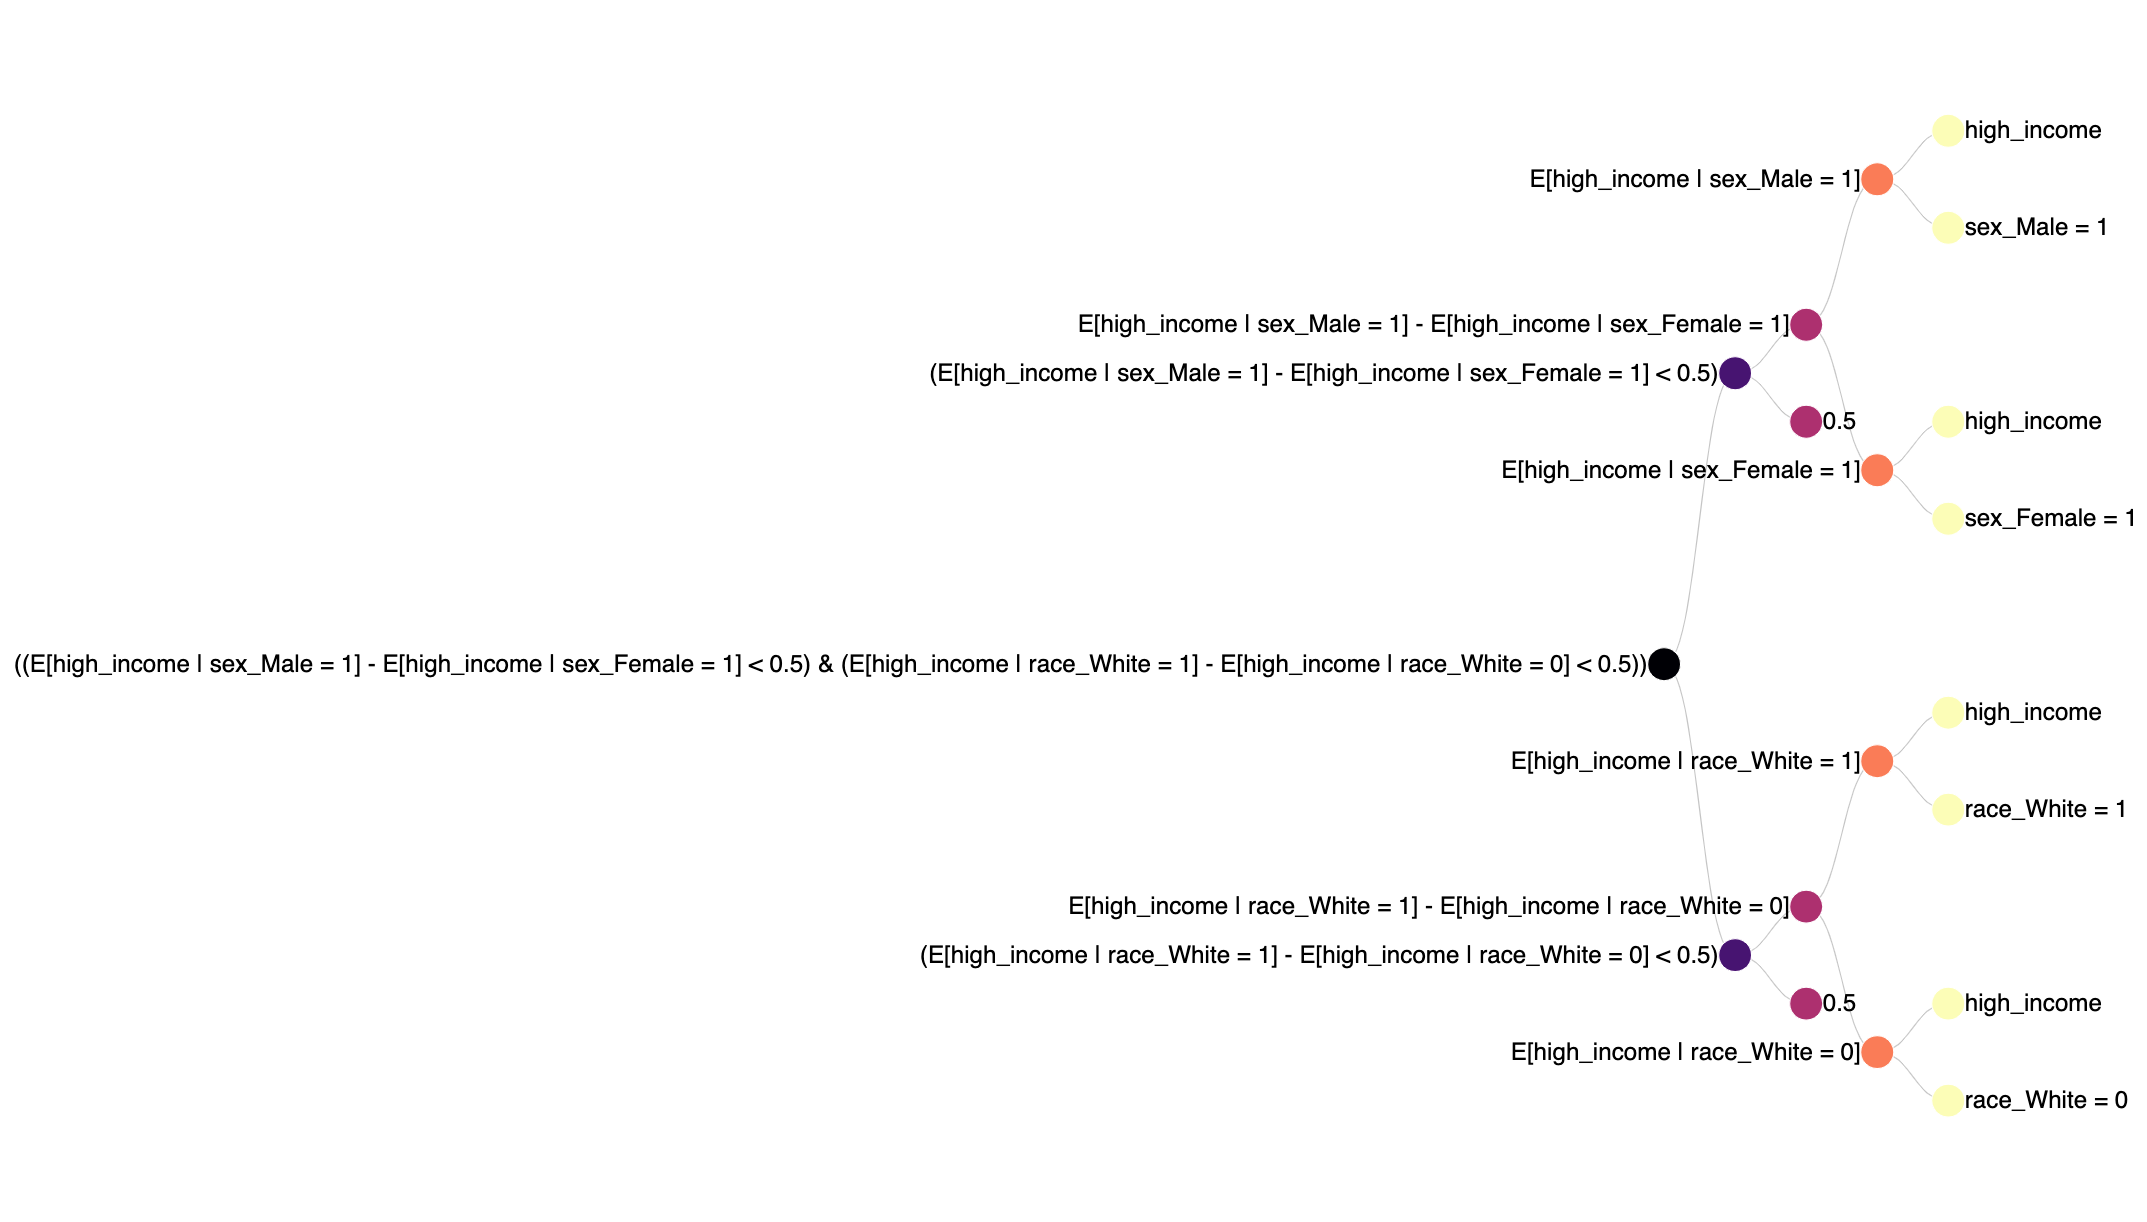
\includegraphics[angle=90,width=0.5\textwidth]{avoir/images/adult-spec-tree-initial.png}
    \caption{Tree of initial specification before refinement in the adult income dataset.}
    \label{fig:casestudy:adult:initial-spec}
\end{figure}
Figure~\ref{fig:casestudy:adult:initial-spec} shows a subtree of the specification visualized through Vega.
A developer analyzing this spec can click on the top pink node to see the evolution of the sex fairness part of the specification and superimpose the threshold.
The threshold is set to be evaluated with every 5 new data points added to the materialized view.
Clicking on the corresponding element in the right subtree, the developer can see Figure~\ref{fig:casestudy:adult:specplot:right}. 


\subsection{COMPAS Risk Assessment via Materialized Views}
The Correctional Offender Management Profiling for
Alternative Sanctions (COMPAS) recidivism risk score data is a popular dataset for assessing machine bias of commercial tools used to assess a criminal defendant's likelihood to re-offend.
The data is based on recidivism (re-offending) scores derived from a software released by Northpointe and widely used across the United States for making sentencing decisions.
In 2016, \citet{angwin2016machine} released an article and associated analysis code critiquing machine bias associated with race present in the COMPAS risk scores for a set of arrested individuals in Broward County, Florida over a period of two years.
The analysis concluded that there were significant differences in the risk assessments of African-American and Caucasian individuals.
Northpointe pushed back in a report~\citep{dieterich2016compas} strongly rejecting the claims made by the ProPublica article; instead, they claimed that \citet{angwin2016machine} made several statistical and technical errors in the report.
In this case study, we use \AVOIRmethodname{} to study the claims made by the two aforementioned reports. 
First, we start with the data released by ProPublica and load it into a pandas-simulated DB.
We then create a materialized view that corresponds to the preprocessing steps used in the publicly available ProPublica analysis  notebook\footnote{https://github.com/propublica/compas-analysis}.
We look at ``Sample A''~\citep{dieterich2016compas}, where the analysis of the ``not low'' risk assessments using a logistic regression model reveals a high coefficient associated with the factor associated with race being African-American.
In terms of a fairness metric, this corresponds to false positive rate (FPR) balance (predictive equality)~\citep{verma2018fairness} metrics. 
The associated specification in \AVOIRmethodname{} grammar would be

\begin{lstlisting}[columns=flexible, language=Python]
   E[hrisk | race=African-American & recid=0] / 
   E[hrisk | race=Caucasian & recid=0] < 1.1
\end{lstlisting}

Where \verb|hrisk| is an indicator for high risk assessments made by the \emph{black-box} COMPAS tool as defined by ~\citet{angwin2016machine},  \verb|recid| is an indicator for re-offending within 2 years of first arrest, and a $10\%$-rule is used as the threshold. 
We choose a failure threshold probability of $\Delta = 0.1$, with the optimization run after every batch of $5$ samples.
\AVOIRmethodname{} finds that when the decisions are made in a sequential, online fashion, the assertion for violation of the specification cannot be made with the required failure guarantee.

By analyzing the components using the visualization tool, one can glean that \AVOIRmethodname{} is unable to optimize since the lower FPR in the denominator (FPR for Caucasian individuals) increasing the overall variance and limiting the ability to optimize for guarantees. 
We follow this analysis by using the reciprocal specification, i.e.,
\begin{lstlisting}[columns=flexible, language=Python]
   E[hrisk | race=Caucasian & recid=0] /
   E[hrisk | race=African-American & recid=0] > 0.9
\end{lstlisting}

we find that indeed, the specification is violated with a confidence of over $1 - \Delta = 0.9$ probability, and \AVOIRmethodname{} can detect this violation within about half the number of available assessments (3350 steps) when run in an online setting.
Figure~\ref{fig:casestudy:compas:propublica} demonstrates the progression of the tracked expectation term. 
Thus, if deployed with the corrected specification, \AVOIRmethodname{} would be able to alert Northpointe of a violation/potentially-biased decision making tool.

\begin{figure}[ht!]
    \begin{subfigure}{0.45\linewidth}
        \centering
        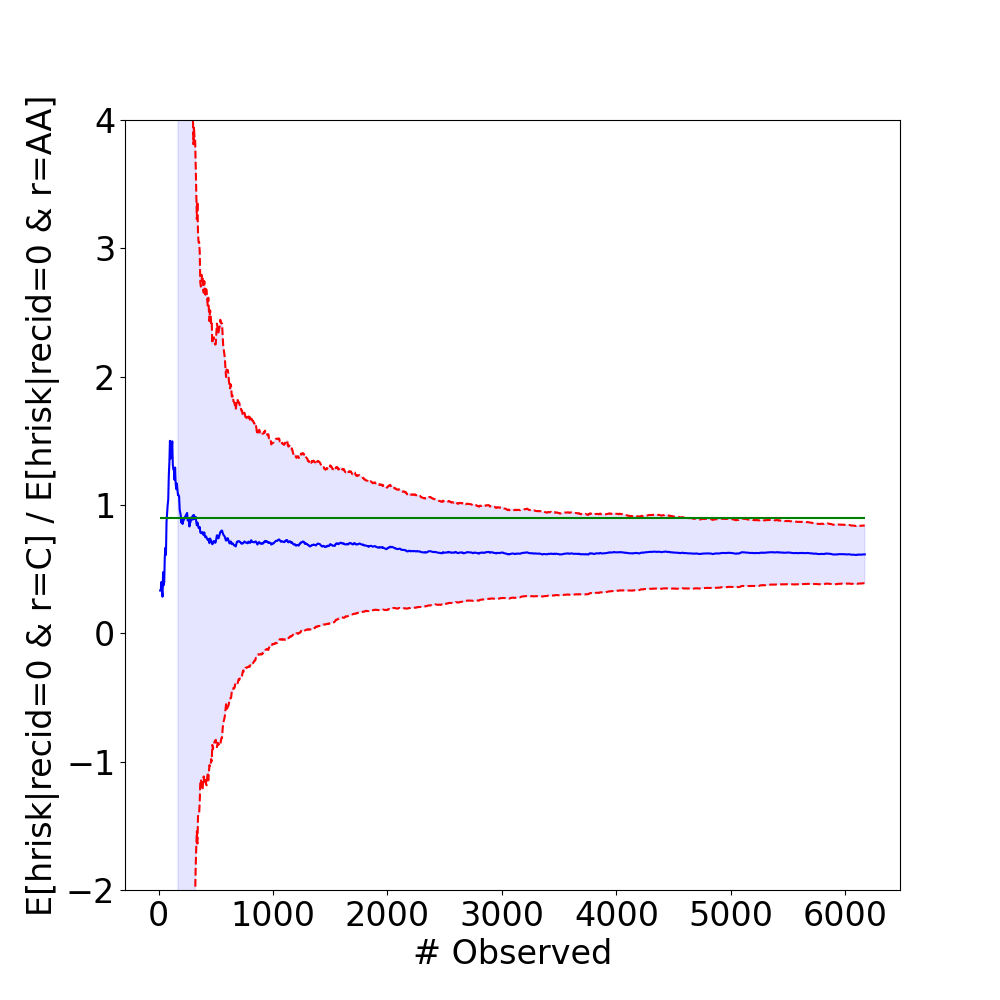
\includegraphics[width=\linewidth]{avoir/images/compas-propublica-et.png}
        \caption{(ProPublica) COMPAS, ``Sample A'' False Positive Rate Bias specification required to \emph{above} the $10\% \implies 0.9$ threshold converges to a value that can be guaranteed to be \emph{under} the required threshold.}
        \label{fig:casestudy:compas:propublica}
    \end{subfigure}
    \hfill
    \begin{subfigure}{0.45\linewidth}
        \centering
        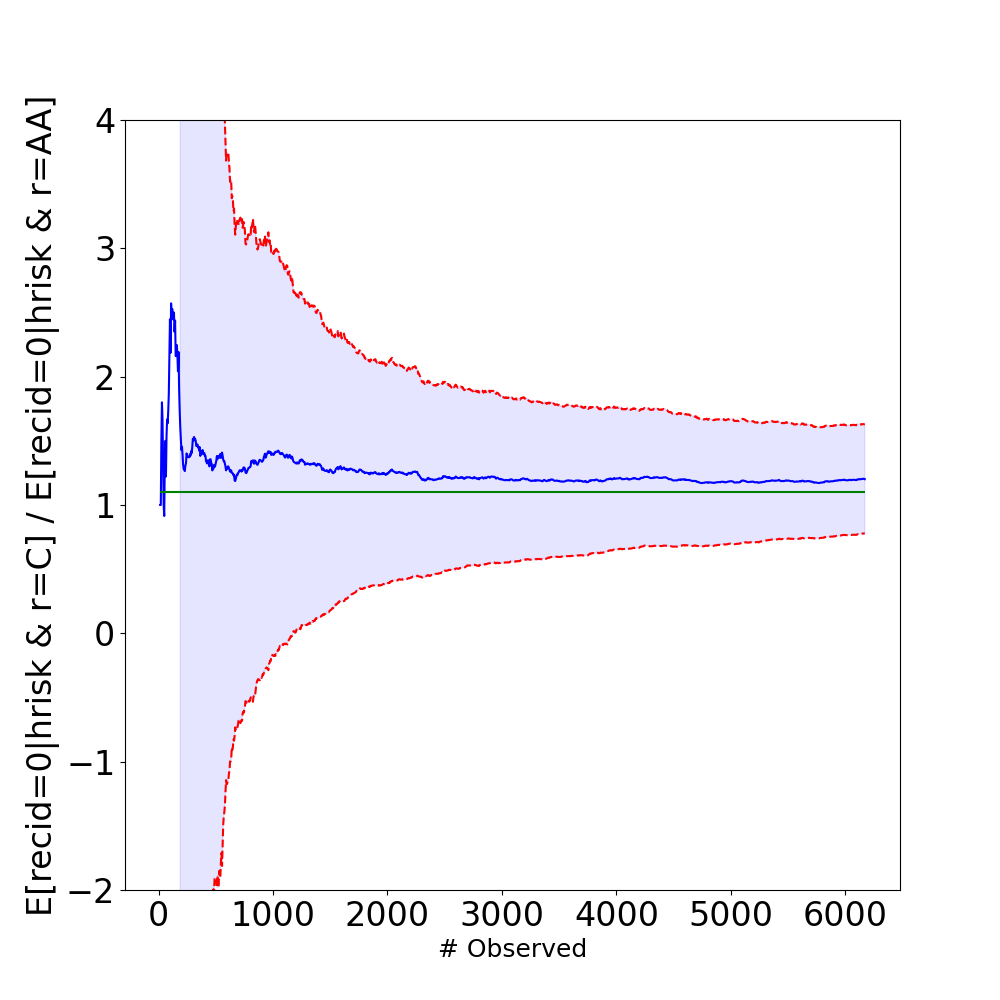
\includegraphics[width=\linewidth]{avoir/images/compas-northpointe-et.png}
        \caption{(Northpointe) ``Sample B'' analysis done by Northpointe  using False Discovery Rate that opposed the ProPublica reports.}
        \label{fig:casestudy:compas:northpointe}
    \end{subfigure}
    \caption{COMPAS dataset case study.}
\end{figure}


The Northpointe report~\citep{dieterich2016compas} makes several claims about the shortcomings of this analysis, but one of the primary claims is that \citet{angwin2016machine} used an analysis based on ``Model Errors'' rather than ``Target Population Errors''.
In Fairness metric terms, this refers to the difference between a False Positive Rate (FPR) balance vs False Discovery Rate (FDR) balance, i.e. balancing for predictive parity over predictive equality. 
In probabilistic terms, the difference amounts to comparing $P(\hat{Y} = 1 | Y = 0, g=1, 2)$ (FPR) vs $P(Y = 0 | \hat{Y} = 1, g=1, 2)$ (FDR), where $\hat{Y}$ refers to the decision made by the algorithm, $Y$ refers to the true value, and $g = 1, 2$ reflects group membership~\citep{verma2018fairness}.
This analysis is run on the dataset subset dubbed ``Sample B''.
To test their hypothesis, we run reproduce the corresponding preprocessing steps and run both versions (numerator and denominator being Caucasian) versions of the corresponding specification under the same setup as earlier. 
We find that despite the point estimate being within the required threshold, neither version can be guaranteed with the required confidence with the given data.
Due to paucity of space, we describe only one of the two variants with the corresponding figure (Figure~\ref{fig:casestudy:compas:northpointe}).
\begin{lstlisting}[columns=flexible, language=Python]
   E[recid=0 | race=Caucasian & hrisk] /
   E[recid=0 | race=African-American & hrisk] > 0.9
\end{lstlisting}


We note that the Northpointe report~\citep{dieterich2016compas} does not provide confidence intervals for their claim either. 
Further, even though the report does not release associated code, the point estimates of the False Discovery Rates (FDRs) match those present in the report which increases our confidence in our \AVOIRmethodname{}-based analysis. 

The back and forth exchange has been the subject of much discussion in both academic and journalistic publications~\citep{feller2016computer, washington2018argue}.
Seminal work by \citet{kleinberg2017inherent} proved the impossibility of simultaneously guaranteeing certain combinations of fairness metrics.
While \AVOIRmethodname{} cannot solve this problem, its usage can help provide explicit guarantees on defined metrics.
The specification grammar also provides a simple mechanism for independent replication of claims. 
We conclude this case study by noting that \AVOIRmethodname{} lends itself to successful analysis that is not possible with the Verifair implementation available online. %Importantly, this case study also demonstrates that  \AVOIRmethodname{}, can be directly integrated with database-centric materialized views. 

\begin{comment}
\section{Related work from Databases}
In the database literature researchers~\cite{Nargesian21}, have explored an approach to tailoring data integration strategies to ensure that the data set used for analysis has an appropriate representation of relevant (demographic) groups and it meets desired distribution requirements. The authors describe how to acquire such data in an approximate cost-optimal manner for several realistic settings. This work is orthogonal to our work and yet AVOIR can potentially integrate with the authors approach to examine if fairness criteria are being met during the integration process. In other studies on fairness researchers~\cite{Yang2018,Asudeh19a,Asudeh19b}, have considered the problem of personalized fair ranking functions and discuss approaches to determine if a proposed ranking function satisfies a set of  desired fairness criteria and, if it does not, to suggest modifications that do. AVOIR attempts to solve a  more general purpose problem (not limited to any particular fairness criteria) and is agnostic to the specific model (treats it as a blackbox).  While we have not examined the performance of AVOIR for fair ranking problems, it is something we plan to examine in the future.
\end{comment}

\section{Supported Metrics}
\label{sec:appendix:additional-metrics}

\begin{table}[ht]
    \centering
    \resizebox{\linewidth}{!}{
    \begin{tabular}{lcc}
    \toprule
        Metric Name  & Definition & DSL  \\
    \midrule \\
       Statistical Parity  & \multirow{2}{*}{$\Pr[d=1|G=m] = \Pr[d=1|G=f]$}  & \multirow{2}{*}{$\E[d|G=m] / \E[d|G=f] < c$} \\
       \citep{dwork2012fairness} & &\\
       Predictive Parity & \multirow{2}{*}{$\Pr[Y=1|d=1, G=m] = \Pr[Y=1|d=1, G=f]$} & \multirow{2}{*}{$E[Y=1|d=1, G=f] - \E[Y=1|d=1, G=m] > c$} \\
       \citep{chouldechova2017fair} & & \\
       Equal Opportunity &\multirow{2}{*}{$\Pr[d=0|Y=1, G=m] = \Pr[d=0|Y=1, G=f]$}  & \multirow{2}{*}{$\E[d=0|Y=1, G=m] - \E[d=0|Y=1, G=f] < c$} \\
       \citep{hardt2016equality} & &  \\
       Equalized Odds & $\Pr[d=1|Y=i, G=m] = \Pr[d=1]Y=i, G=f],$ & $(\E[d=1|Y=1, G=f] - \E[d=1|Y=1, G=m] > c_1) \&  $ \\
       \citep{hardt2016equality} & $i = 0, 1$ & $(\E[d=1|Y=0, G=f] - \E[d=1|Y=0, G=m] > c_2)$\\
    \bottomrule
    \end{tabular}
    }
    \caption{Examples of supported metrics.}
    \label{tab:appendix:supported-metrics}
\end{table}

We provide a non-exhaustive list of statistical group-based fairness criteria and show an exact/approximate equivalent in the \AVOIRmethodname{} DSL in Table~\ref{tab:appendix:supported-metrics}.
We use the following notation, adapted from \citet{verma2018fairness}:
\begin{itemize}
    \item[$G$:] Protected or sensitive attribute. For demonstration purposes, we will use the values $m$ and $f$ to denote majority and minorty classes.
    \item[$X$:] Features describing each individual 
    \item[$Y$:] True label for $X$
    \item[$S$:] Probability $\Pr[Y|X, G]$ predicted for a certain class $c$
    \item[$d$:] Predicted decision for $X$, usually derived from $X$
    \item[$c$:] A threshold to test the specification. For ratios based approximations, this would be a number $1 \pm \eps$ for some small $\eps > 0$. For difference based approxiamtions, this number would be some small $\eps > 0$. When multiple terms are present, we use $c_i$ to denote the $i^{\text{th}}$ threshold.
\end{itemize}
\todo{New section}
We assume that the decision function $f$ tracked by \AVOIRmethodname{} as a signature that takes $X, G, Y$ as input and produces $S$ or $d$ as output.
Note that in their python implementation, $=$ would be replaced by \lstinline{==} and $|$ by the \lstinline{given} keyword.
